\section{Experiment Setup}
\label{s:Experiment-Setup}

This Chapter introduces the experimental measurements of the performance of the Anomaly Detection model presented in Chapter [ref].
The goal is to measure the performances of the A.D. method against the LiMa technique described in [ref] to perform source detection. The sooner a detection is issued, the sooner other observatories can study the same source, enabling the multi-wavelength approach introduced in Chapter 2 [ref]. For this reason, we are interested in measuring how fast the methods are to issue 5$\sigma$ detections.
In addition, we need to perform these measurements for the two scientific use cases of serendipitous discoveries and science alert reactions. In the serendipitous discoveries settings, a GRB appears in the telescope's field of view; hence the totality of the event is observed. When the observatory reacts to a science alert, its telescopes will change their pointing to observe a sky region in which the GRB event is already started. The time taken to change the pointing is considered fixed and equal to 30 seconds. Two test sets of different difficulties have been generated for this purpose.

\subsection{Dataset Generation for performance evaluations}
\label{s:Experiment-Data}
Two supervised datasets of simulated GRB signals have been generated. As stated in Chapter 2, gamma-ray transients differ among several factors: [TODO]. The max flux parameter constrains the maximum luminosity of the phenomena. If the signal is too low, it will be indistinguishable from the noise. The mean of the background signal will be the reference point to tune the difficulty of the problem and it is defined by the same IRF used in the training test generation ($North\_z40\_5h\_LST$), described in Chapter .. [ref]. Figure~\ref{f:exp-max-flux-distribution-E} show that the first dataset (called $E=easy$) contains GRB simulated trials with a max flux greater or equal to the mean of the background signal. It contains 1 trials with a max flux in the interval $[1.2264e-09, \infty]$]. In the second dataset (called $H=hard$), the max flux goes down to 1$\sigma$ below the background threshold. It contains 438 trials with a max flux in the interval $[2.6785e-10, \infty]$].  

%The simulation tool can use this parameter to generate samples with different luminosity.  

\begin{figure}[t]
\centering
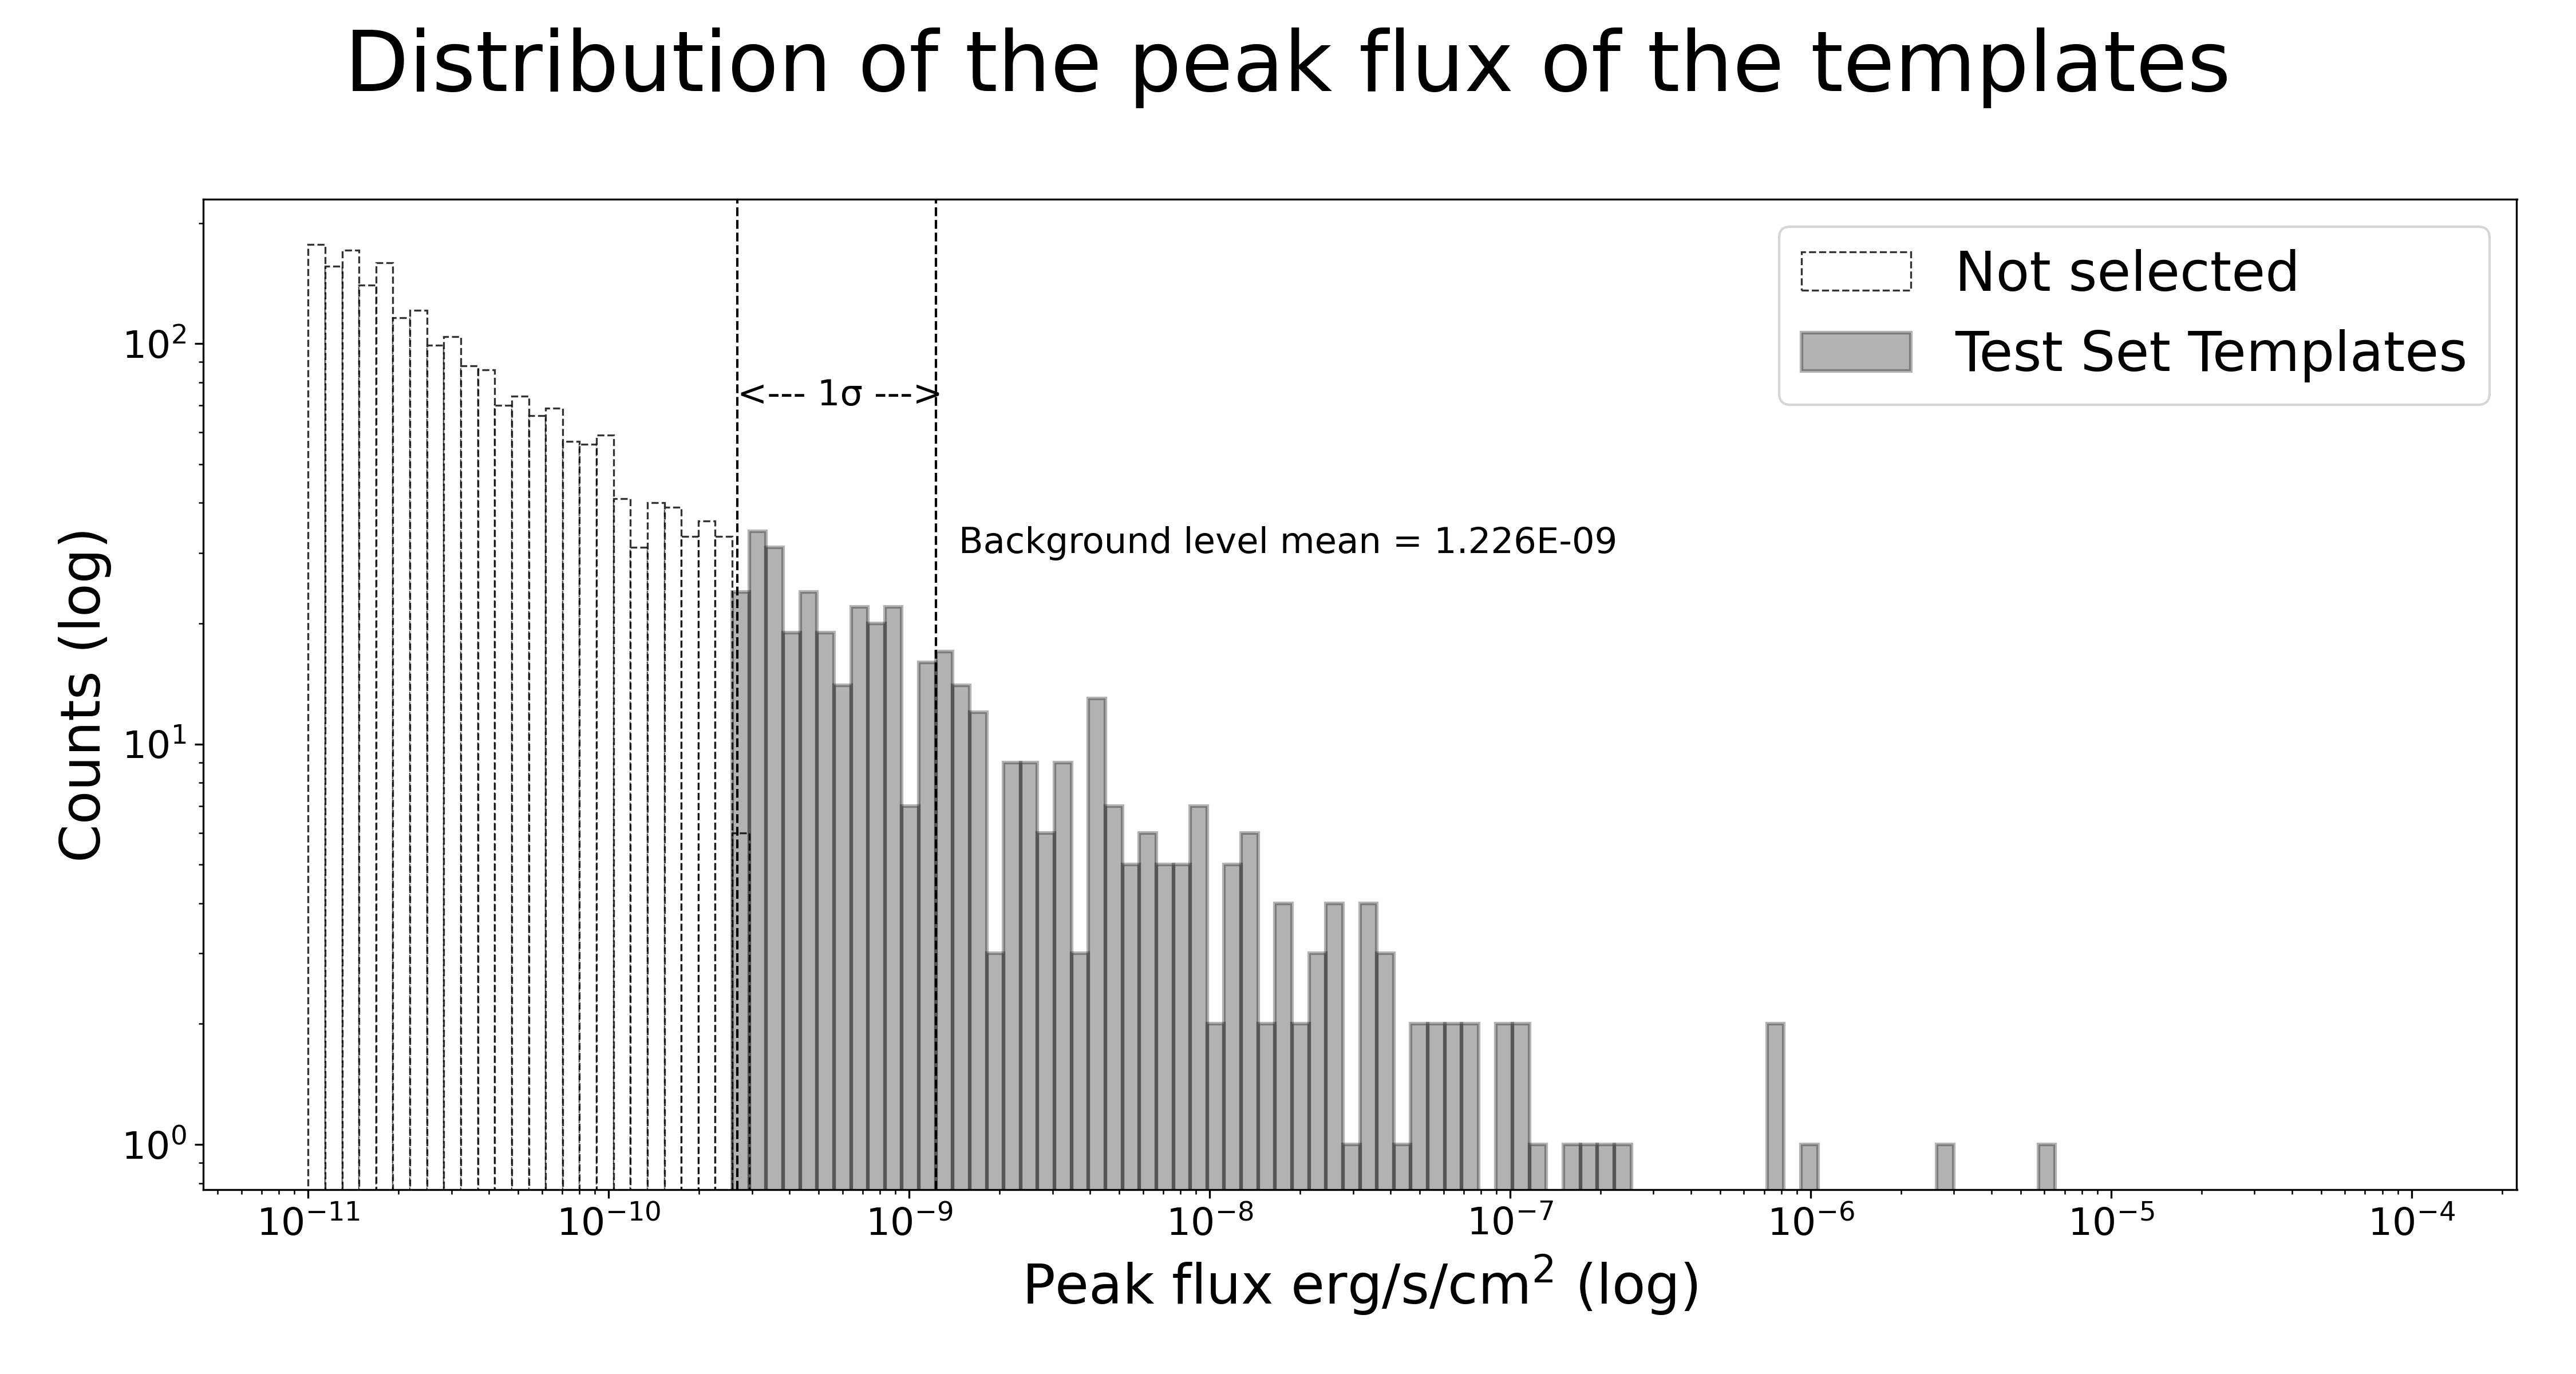
\includegraphics[width=1\textwidth]{figures/experiments/templates_max_flux_distributions.png}
\caption{The distribution of the maximum flux for each GRB template. The test sets E and H contain respectively 188  and 438 of GRB simulated trials, and their maximum fluxes are within: $[[1.2264e-09, \infty]]$ and $[[2.6785e-10, \infty]]$.}
\label{f:exp-max-flux-distribution-E}
\end{figure}


The simulation time is limited to 500 seconds because we are interested in the first part of the signal, given the nature of the scientific use cases described in Chapter [ref]. The trigger time that defines the GRB event's start is 250 seconds. The integration time is the same used for the training set generation for the reasons stated in Chapter [ref]. The autoencoder models have been trained with time series of lengths equal to 5, with each point being a flux measurement integrated in 5 seconds. Hence the same settings are used here. The stride parameter is set to 1 because this method can work with temporal bins that are statistically dependent, and this drastically reduces the time the model takes to wait for data during the online inference. Table [ref] summarizes the configuration parameters described above. A time series is labeled as anomalous if contains at least one point of GRB signal. Figure [ref] shows some samples of GRB simulated trials.  


%\subsection{Environment and System Setup}
%\label{s:Experiment-Env}
%agilehost3.. 

\section{Results}
\label{s:Experiment-Results}

\subsection{Serendipitous discoveries use case}
\label{s:Serendipitous-Discoveries-Results}

\begin{table}[!htb]
    \begin{minipage}{.5\linewidth}
      \centering
        \begin{tabular}{|lll|}
        \hline
        \rowcolor[HTML]{EFEFEF} 
        \multicolumn{3}{|c|}{\textbf{Test set E}}  \\ \hline
        \multicolumn{1}{|l|}{\textbf{Model}} & \multicolumn{1}{l|}{\textbf{A.D.}} & \textbf{Li\&Ma} \\ \hline
        \multicolumn{1}{|l|}{\textbf{Total detections}}       & \multicolumn{1}{l|}{141}           & 179             \\ \hline
        \multicolumn{1}{|l|}{\textbf{Avg time (s)}} & \multicolumn{1}{l|}{48.16}         & 60.75           \\ \hline
        \end{tabular}
    \end{minipage}%
    \begin{minipage}{.5\linewidth}
      \centering
        \begin{tabular}{|lll|}
        \hline
        \rowcolor[HTML]{EFEFEF} 
        \multicolumn{3}{|c|}{\textbf{Test set H}}  \\ \hline
        \multicolumn{1}{|l|}{\textbf{Model}} & \multicolumn{1}{l|}{\textbf{A.D.}} & \textbf{Li\&Ma} \\ \hline
        \multicolumn{1}{|l|}{\textbf{Total detections}}       & \multicolumn{1}{l|}{0}           & 0 \\ \hline
        \multicolumn{1}{|l|}{\textbf{Avg time (s)}} & \multicolumn{1}{l|}{0}         & 0           \\ \hline
        \end{tabular}

    \end{minipage}
       \caption{Total number of 5$\sigma$ detections performed by the two methods of A.D. and LiMa and the average time in seconds the methods took to detect a source for the first time.}
    \label{tab:Experiment-Results-1} 


\end{table}
Table~\ref{tab:Experiment-Results-1} shows the total number of 5$\sigma$ detections performed by the two methods of A.D. and LiMa and the average time in seconds the methods took to detect a source for the first time. This time is measured starting from the trigger time that defines the start of the GRB event and not from the start of the observation.

The table shows the LiMa's robust predictions since it detected most GRBs. The A.D. method performs less robust but faster detections since it can predict every $T$ seconds. In LiMa the temporal bins must be independent and the slower prediction rate is 1  every $T*TSL$ seconds. This metric can be broken down further. 
\begin{figure}[t]
\centering
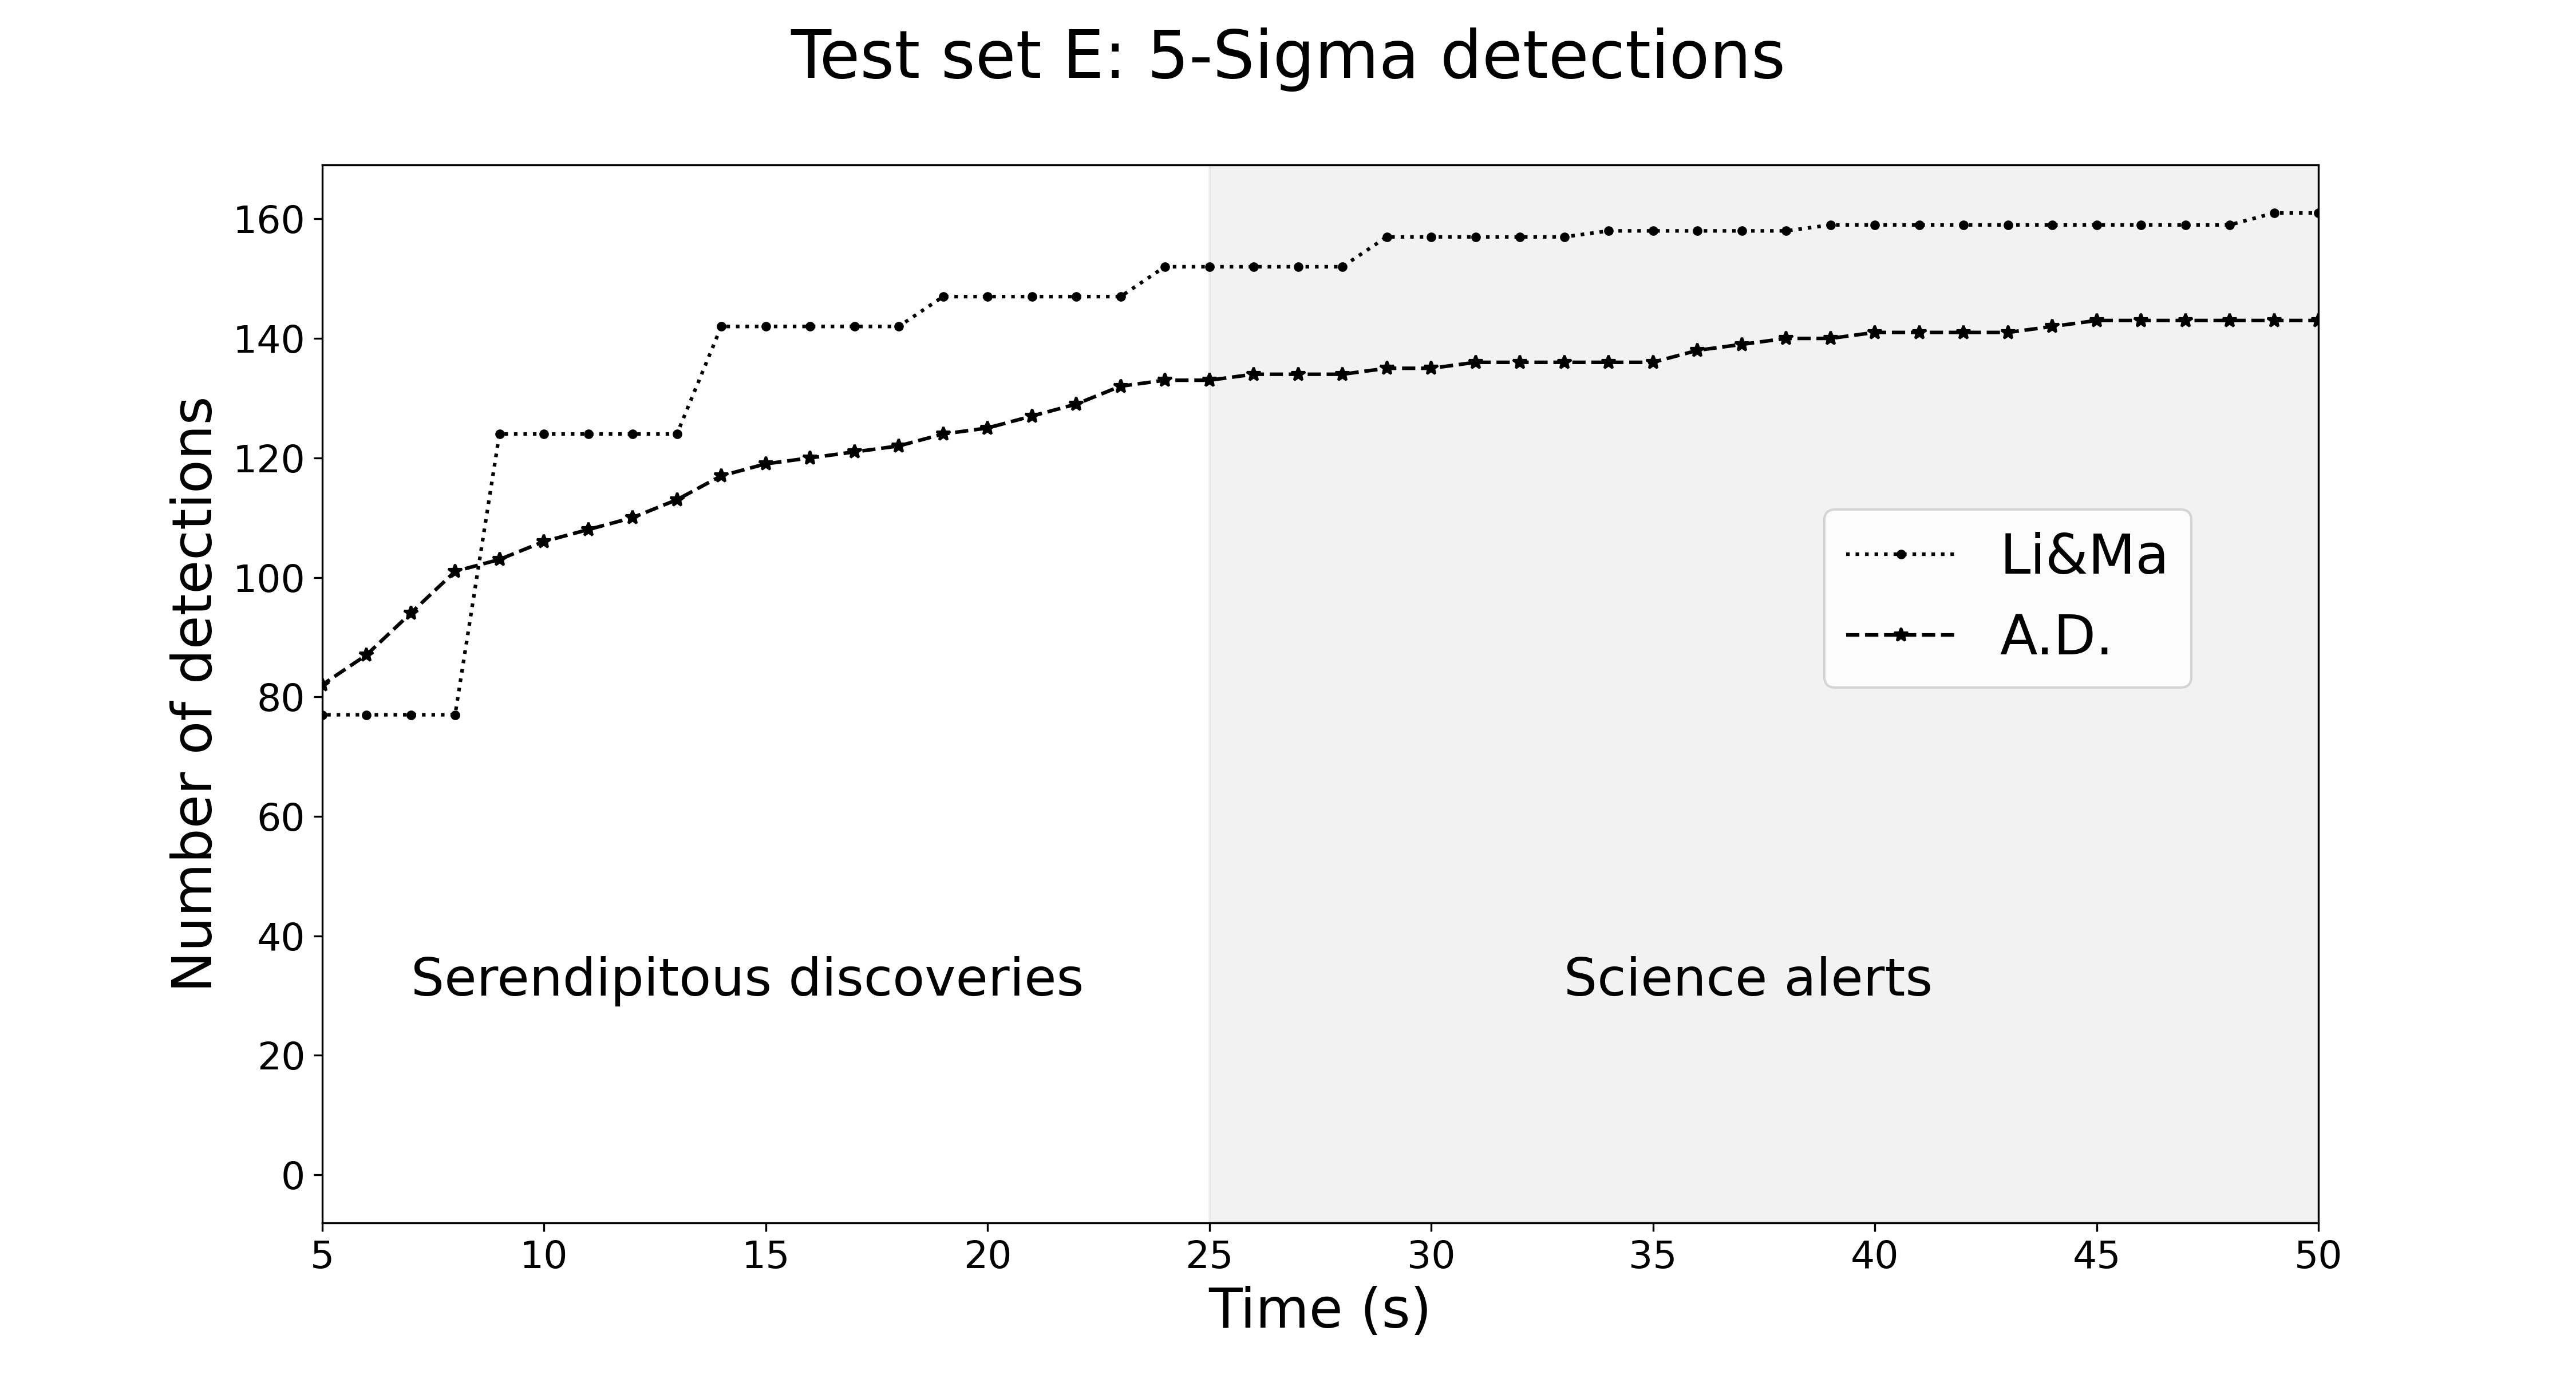
\includegraphics[width=1\textwidth]{figures/experiments/ad_vs_li_ma_testset_e.png}
\caption{Result on Test Set E: Total number of 5$\sigma$ detections (out of 188) performed by the two methods of A.D. and LiMa in the time-constrained requirements. }
\label{f:ad-vs-lima}
\end{figure}



\begin{table}[!htb]
    \begin{minipage}{.5\linewidth}
      \centering
        \begin{tabular}{lllll}
        \hline
        \rowcolor[HTML]{EFEFEF} 
        \multicolumn{5}{c}{\textbf{Test set E}} \\ 
        \hline
        \multicolumn{1}{|l|}{\textbf{Tmax (s)}} & \multicolumn{1}{l|}{\textbf{5}} & \multicolumn{1}{l|}{\textbf{10}} & \multicolumn{1}{l|}{\textbf{25}} & \multicolumn{1}{l|}{\textbf{50}}  \\ \hline
        \multicolumn{1}{|l|}{\textbf{Td A.D.}} & \multicolumn{1}{l|}{9} & \multicolumn{1}{l|}{21} & \multicolumn{1}{l|}{60} & \multicolumn{1}{l|}{92}  \\ \hline
        \multicolumn{1}{|l|}{
            \textbf{Td LiMa}} & \multicolumn{1}{l|}{0} & \multicolumn{1}{l|}{0}  & \multicolumn{1}{l|}{79} & \multicolumn{1}{l|}{128} \\ \hline
        \end{tabular}        
    \end{minipage}
    \begin{minipage}{.5\linewidth}
      \centering
        \begin{tabular}{lllll}
        \hline
        \rowcolor[HTML]{EFEFEF} 
        \multicolumn{6}{c}{\textbf{Test set H}} \\ 
        \hline
        \multicolumn{1}{|l|}{\textbf{Tmax (s)}} & \multicolumn{1}{l|}{5} & \multicolumn{1}{l|}{10} & \multicolumn{1}{l|}{25} & \multicolumn{1}{l|}{50}   \\ \hline
        \multicolumn{1}{|l|}{\textbf{Td A.D.}} & \multicolumn{1}{l|}{5} & \multicolumn{1}{l|}{21} & \multicolumn{1}{l|}{60} & \multicolumn{1}{l|}{92}  \\ \hline
        \multicolumn{1}{|l|}{\textbf{Td LiMa}} & \multicolumn{1}{l|}{0} & \multicolumn{1}{l|}{0}  & \multicolumn{1}{l|}{79} & \multicolumn{1}{l|}{128} \\ \hline
        \end{tabular}        
       \caption{}    
    \end{minipage}
   \caption{Total number of 5$\sigma$ detections performed by the two methods of A.D. and LiMa in the time-constrained requirements.}    
    \label{tab:Experiment-Results-2} 
\end{table}

\begin{figure}[t]
\centering
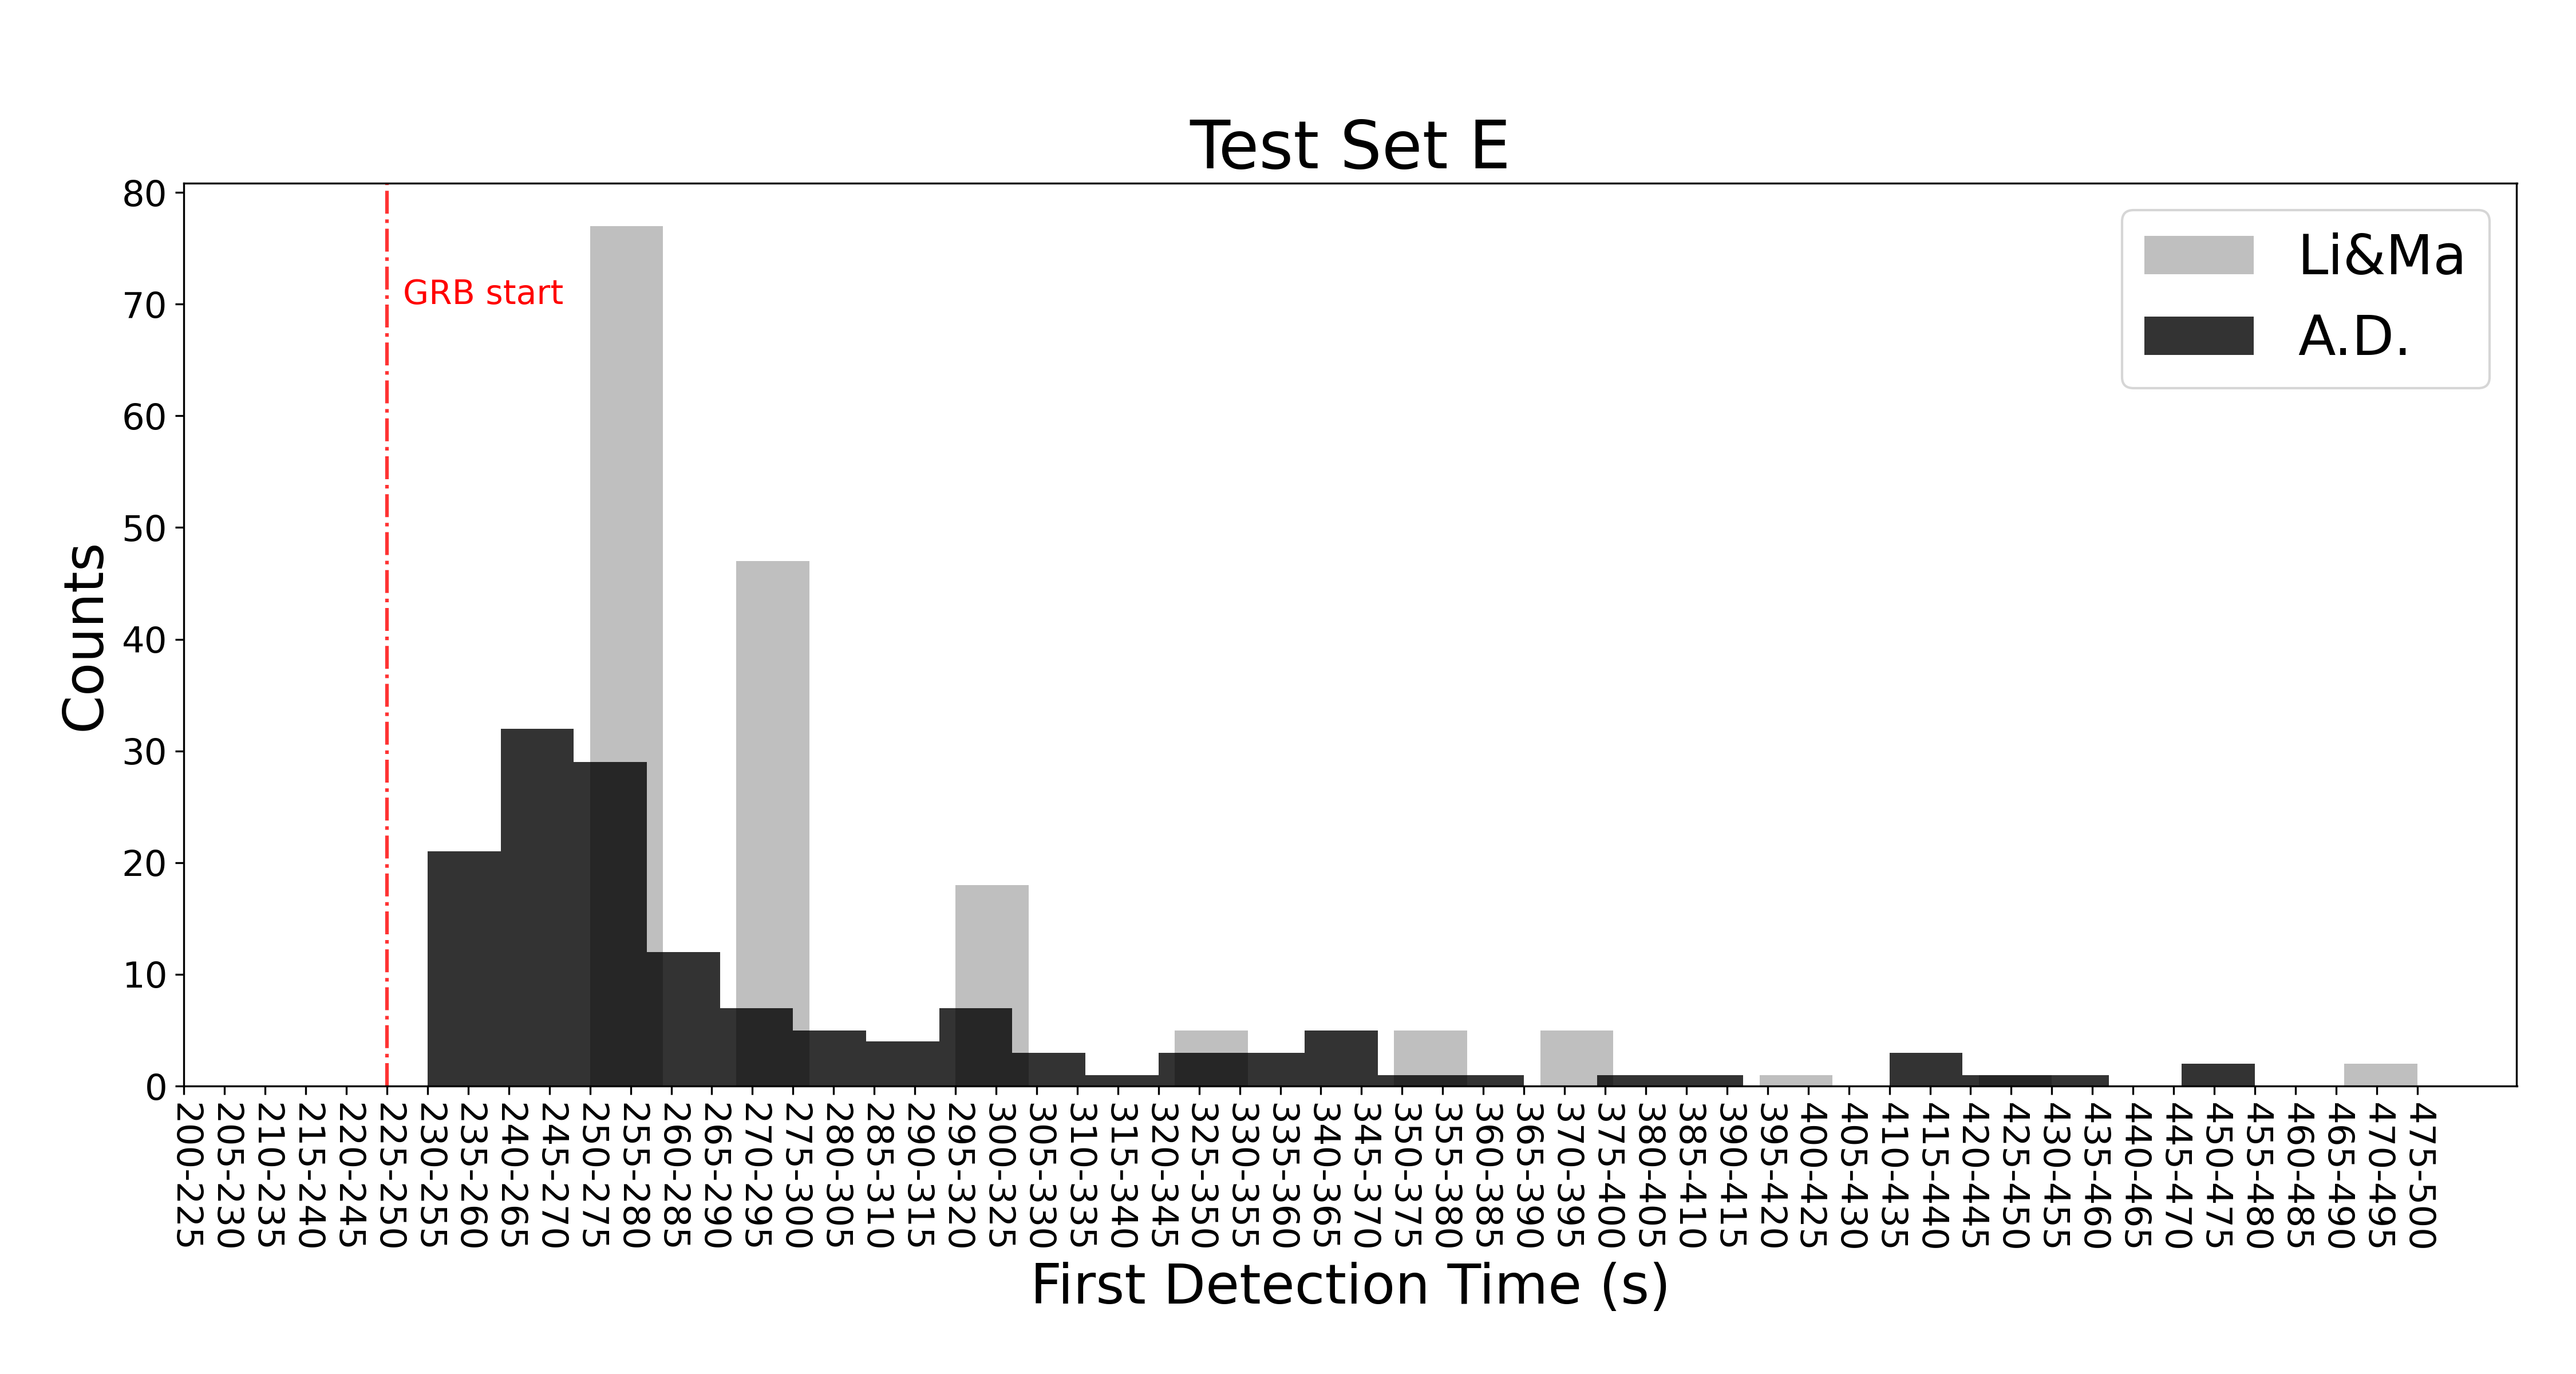
\includegraphics[width=1\textwidth]{figures/experiments/ad_vs_li_ma_first_detections_testset_e.png}
\caption{Result on Test Set E: 5$\sigma$ detection times distributions for A.D. and LiMa over GRB 188 trials.}
\label{f:ad-vs-lima-first-detection}
\end{figure}


Table~\ref{tab:Experiment-Results-2}, Fig~\ref{f:ad-vs-lima-first-detection} and Fig~\ref{f:ad-vs-lima} shows the number of predictions at shorter time scales, limiting the duration of the observation. 
% Li&Ma è nel caso peggiore ovvero il bin temporale non sta mai a cavallo dell'onset
The A.D. method is capable of faster prediction on the very short-term temporal scale.  












\subsection{Science alert use case}
\label{s:Science-Alert-Results}
The science-alert use case further limits the time domain. When the observatory reacts to a science alert, its telescopes will change their pointing to observe a sky region in which the GRB event is already started. The time taken to change the pointing is considered fixed and equal to 30 seconds.  


\section{Summary}
\label{s:Experiments-Summary}

Summarize the key findings of the experiments you conducted.
